\section{Deep learning}
Die Begriffe \textit{Deep Learning}, \textit{maschinelles Lernen} und \textit{künstliche Intelligenz} werden oft fälschlicherweise austauschbar verwendet. Es gibt allerdings eine ganz klare, und für das Verständnis wichtige Hierarchie zwischen den Begriffen. Um Klarheit zu verschaffen werden darum alle Gebiete aufgeführt. Die folgende Abbildung zeigt den hierarchischen Zusammenhang der Begriffe.

\begin{figure}[hbt]
	\centering
		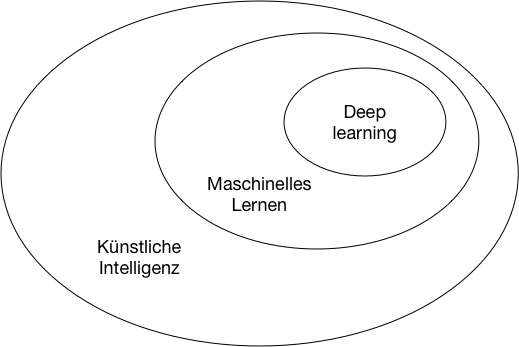
\includegraphics[width=0.6\textwidth]{assets/hierarchy.png}
	\caption{Künstliche Intelligenz, Maschinelles Lernen und Deep Learning}
	\label{img:hierarchy}
\end{figure}

Das Gebiet der künstlichen Intelligenz gibt es schon so lange wie den Computer selbst. Die Frage, wie schlau ein Computer werden kann, beschäftigt uns bis heute. Als anerkannte Definition für KI gilt, das Bestreben intellektuelle Aufgaben, die normalerweise von Menschen gelöst werden, zu automatisieren \parencite[][Kap. 1.1.1]{chollet}.\index{Künstliche Intelligenz (KI)}

Erste Erfolge erreichte man zum Beispiel mit Schachcomputern, die handgeschriebene Regeln befolgten. Diese Form von künstlicher Intelligenz hat aber schnell Grenzen, da die Lösungen vieler Prozesse schlicht zu komplex sind, um sie unter angemessenem Aufwand mit Regeln zu beschreiben. Mit der Zeit verbreitete sich darum eine neue Methode: Maschinelles Lernen.\index{Maschinelles Lernen} \parencite[vgl. ][Kap. 1.1.1]{chollet}

Der Ablauf von maschinellem Lernen ist grundlegend anders als konventionelles Programmieren. Der Entwickler muss keinen Programmcode mit festen Regeln schreiben, im Gegenteil: Er liefert dem Computer Trainigsdaten, und der Computer lernt die Regeln selbst. Die bekannteste Kategorie von Machine Learning Algorithmen ist \textit{Überwachtes Lernen}. Bei überwachtem Lernen bestehen die Trainingsdaten aus Eingaben $x$ und zugehörigen Ausgaben $y$. Der Algorighmus versucht die Abbildungsfunktion $f$ zwischen den Eingaben und den Ausgaben zu bestimmen. 
$$ y = f(x)$$
Der Name \textit{Überwachtes Lernen} kommt daher, dass man sich den Lernalgorithmus wie einen Lehrer vorstellen kann der die Abbildungsfunktion überwacht. Die korrekten Ausgaben zu den Eingaben sind bekannt. Die Abbildungsfunktion berechnet iterativ Ausgaben zu den Trainingsdaten und der Lernalgorithmus korrigiert ihn mit den Lösungen. Der Lernprozess hört auf sobald die Abbildungsfunktion soviel wie möglich gelernt hat. Kurzgesagt lernt das System aus, Beispielen Muster zu erkennen. Dieser Prozess wird \textit{Training} genannt. Maschinelles Lernen blühte erst in den 90'er Jahren auf, wurde aber schnell zum grössten Teilgebiet der künstlichen Intelligenz. \parencite[vgl. ][Kap. 1.1.2]{chollet} \parencite[vgl. ][]{supervised}

Beim maschinellem Lernen, lernt die Software im Grunde eine nützlichere Darstellungsweise der Daten bzw. der Eingabe. Anhand dieser anderen Repräsentation kann der Computer die Antwort einfach erkennen. Abbildung \ref{img:repr} zeigt als Beispiel  zwei unterschiedliche Repräsentationen von Daten. Um zwischen roten und blauen Elementen zu unterscheiden, ist Repräsentation (c) eindeutig praktischer als (a). Um bei (c) zwischen roten und blauen Elementen zu unterscheiden, gilt einfach: Falls $x>0$ ist das Element blau und sonst ist es rot. Bei Deep Learning gehen die Daten durch eine Folge von aufeinander aufbauenden Repräsentationen. Jede Repräsentation ist ein wenig nützlicher um das Problem zu lösen als die Vorherige.  Auf diese Weise kann der Computer zunehmend komplexe Probleme, in einfacheren Zwischenschritten lösen. Das \textit{Deep} in Deep Learning entspringt der grossen Anzahl an aufeinanderfolgenden Repräsentationen. Die Verbindung zwischen Deep Learning und überwachtem Lernen ist, dass Deep Learning eine Kategorie von Abbildungsfunktionen beschreibt. Deep Learning bezeichnet das Konzept von stufenweisem Lernen und nicht eine einzelne Methode.  Eine weit verbreitete Methode sind allerdings \textit{tiefe künstliche neuronale Netze}. \parencite[vgl.][]{chollet} \index{Deep Learning}

\begin{figure}[hbt]
	\centering
	\begin{subfigure}{0.3\textwidth}
		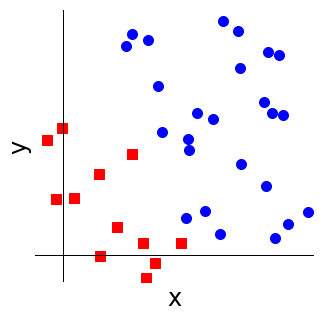
\includegraphics[width=0.9\textwidth]{assets/repr_0.png}
		\caption{Rohe Daten}
	\end{subfigure}
	\begin{subfigure}{0.3\textwidth}
		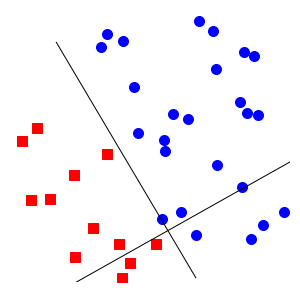
\includegraphics[width=0.9\textwidth]{assets/repr_1.png}
		\caption{Koordinatenwechsel}
	\end{subfigure}
	\begin{subfigure}{0.3\textwidth}
		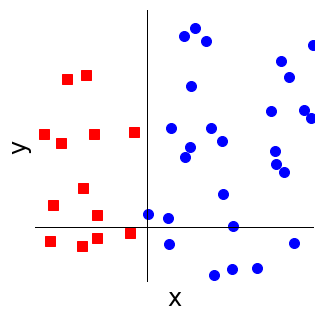
\includegraphics[width=0.9\textwidth]{assets/repr_2.png}
		\caption{Bessere Repräsentation}
	\end{subfigure}
	\caption{Unterschiedliche Repräsentationen}
	\label{img:repr}
\end{figure}

\subsection{Künstliche neuronale Netze}

\textit{Künstliche neuronale Netze} \index{Künstliche neuronale Netze}hat man sich, wie der Name schon preisgibt, von der Natur abgesehen. Ähnlich wie in unserem Gehirn gibt es Neuronen bzw. Knoten und dazwischenliegende Verbindungen. Die \say{Intelligenz} entsteht erst aus dem Zusammenspiel tausender Neuronen. Künstliche Neurone Netze haben sich mittlerweile so stark weiterentwickelt, dass sie nebst der ursprünglichen Idee, nichts mehr mit der biologischen Variante gemeinsam haben. \\

Der Wert eines Knotens/Neurons ist abhängig von der Summe aller seiner eingehenden Verbindungen. Was der Wert einer Verbindung ist wird weiter unter erklärt. Die Abhängigkeit von der Summe wird durch die Aktivierungsfunktion $\sigma$ definiert. Die Aktivierungssfunktion ist wichtig, damit das Netzwerk jede mögliche Funktion abbilden kann. Es ist bewiesen dass neuronalen Netze universelle Approximatoren sind \parencite[][Kap. 4]{universal}. Eine bekannte Aktivierungsfunktion ist zum Beispiel die \textit{ReLU} \index{ReLU}Funktion. Sie wird vor allem für ihre Einfachheit geschätzt. Die ReLU Funktion unterdrückt negative Werte, bzw. sie ist null für Werte kleiner als Null. \parencite[vgl.][]{neuronale_netze}  \parencite[vgl.][]{chollet}
$$\sigma(x) = \text{ReLU}(x) = \text{max}(0, x)$$

Der Wert einer eingehenden Verbindung entspricht dem Produkt des Herkunftsknoten, bzw. des Knoten woher die Verbindung kommt, und dem Gewicht $w \in \mathbb{R}$ der Verbindung. Die Gewichte der Verbindungen sind die Parameter des Netzwerks. Intuitiv kann man sich vorstellen, dass das Netzwerk lernt, wichtigeren Verbindungen höhere Gewichtungen zu geben und Unwichtigen umgekehrt. Wenn man alles zusammensetzt ergibt sich für den Wert irgendeinen Knotens $o_i$ mit Vorgänger-Knoten $\boldsymbol{h}$ diese Formel:
$$ o_i = \sigma\Big(\sum_i h_i \cdot w_{i}\Big)$$
Die fettgedruckte Notation bedeutet, dass ein Vektor gemeint ist. Normal geschriebene Buchstaben mit Index bezeichnen die Komponenten des Vektors. Mit dieser Formel propagieren sich die Werte der Anfangsknoten durch das ganze Netzwerk. Um das Prinzip anschaulicher zu machen, wird ein Beispiel-Durchlauf vorgeführt. Die verwendeten Gewichte und Eingaben sind willkürlich.

Die Aufgabe des vorgestellten Netzwerks ist es zum Beispiel, zwischen Hund und Katze zu unterscheiden. Die Eingaben $x_1$ und $x_2$ sind gewisse Merkmale des zu erkennenden Tieres. $1$ bedeutet, dass Tier besitzt das Attribut und $0$ das Gegenteil. Die Ausgabe $o$ beschreibt die Wahrscheinlichkeit, dass das Tier eine Katze ist. Daraus folgt, dass Werte $o>0.5$ für Katze stehen und Werte $o<0.5$ für Hunde.
\begin{figure}[hbt]
	\centering
		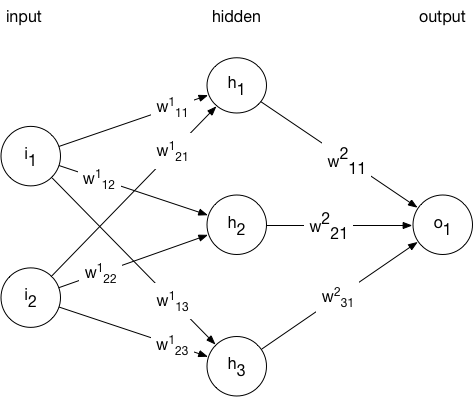
\includegraphics[width=0.85\textwidth]{assets/neural_net.png}
	\caption{Grafische Darstellung eines künstlichen neuronalen Netzwerks anhand eines Beispiels: Rote Zahlen sind festgesetzt und grüne Zahlen werden berechnet.}
	\label{img:neuralnet}
\end{figure}
\\
Die versteckte Schicht ist wichtig damit das Netzwerk eine grössere Anzahl Paramter aus den Daten lernen kann. Je mehr versteckte Schichten es gibt, desto schwierigere Probleme kann das Netzwerk in der Regel lösen. Die Werte jeder versteckten Schichten können als neue Repräsentation der Eingabedaten interpretiert werden. Die Wahl von drei versteckten Knoten im Beispiel ist willkürlich.
\\
Was bis jetzt berechnet wurde, nennt man den \textit{Vorwärtspass}. Aus einer Eingabe wurde die Ausgabe berechnet. Daran war aber noch nichts intelligent. Erst jetzt können die Parameter der Funktion, die Gewichte, aus diesem Beispiel lernen (Siehe Abbildung \ref{img:anatomy}). Um diese zu verbessern, braucht es eine \textit{Verlustfunktion} \index{Verlust Funktion}die uns angibt, wie weit die Ausgabe vom korrekten Ziel entfernt ist. Eine mögliche Verlustfunktion ist die absolute Differenz zwischen dem Ziel und der Ausgabe. Wenn man in oberen Beispiel davon ausgeht, dass die Eingabe wirklich zu einer Katze gehört, ergäbe sich:
$$ \text{Verlust}(output, target) = |target-output| = |1.0-0.747| = 0.253$$
Um den Verlustwert zu minimieren, passt das Netzwerk die Gewichte schrittweise an. Diesen Teil übernimmt der  \textit{Optimierer}. Ein einfacher Optimierer ist zum Beispiel das Gradientenverfahren. Details dazu befinden sich in \parencite{gradient}.

\begin{figure}[hbt]
	\centering
		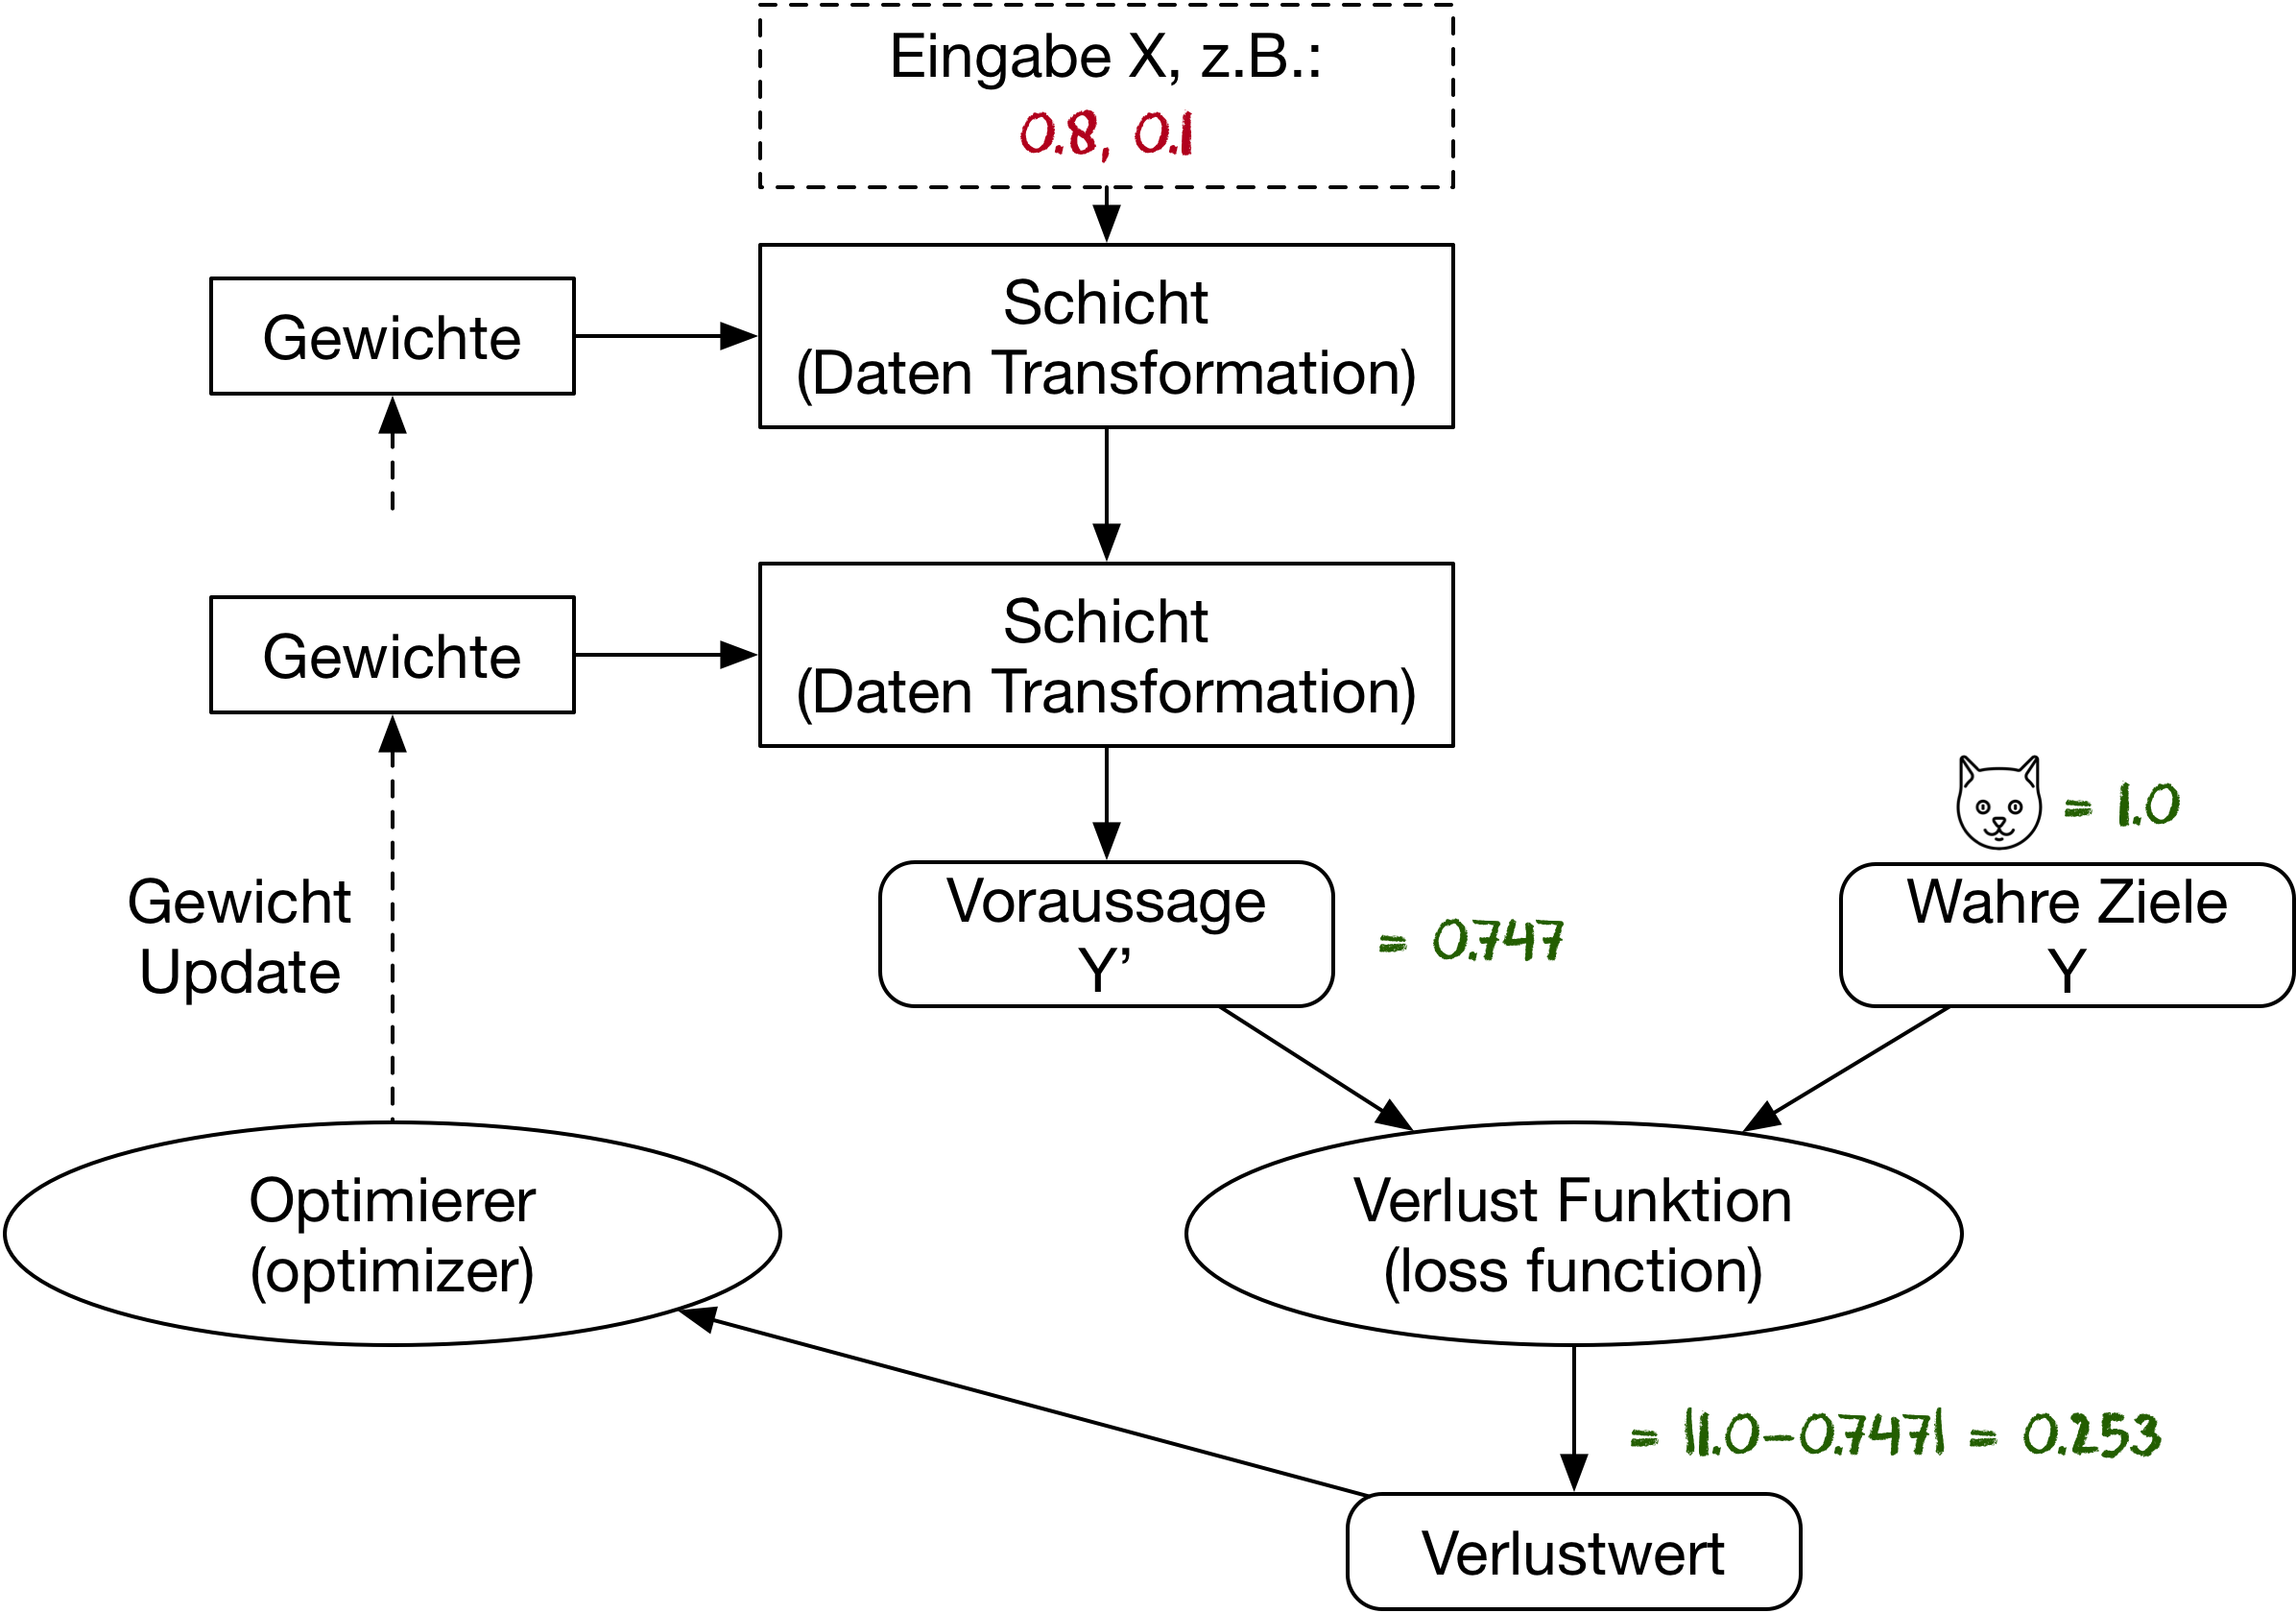
\includegraphics[width=0.8\textwidth]{assets/anatomy.png}
	\caption{Visuelle Darstellung des Lernprozesses anhand eines Beispiels}
	\label{img:anatomy}
\end{figure}

Da bei diesem Typ von neuronalen Netzwerken alle Knoten miteinander verbunden sind, wird es oft \textit{Dense Neural Network} \index{Dense Neural Network}genannt.
\\
Die mathematischen Operationen in einem neuronalen Netzwerk lassen sich alle als Matrizen-Operationen berechnen. Mit Matrizen kann der Computer auf einer Grafikkarte und mit einem \index{BLAS}\textit{BLAS (Basic linear algebra system)} sehr effizient rechnen \parencite{neuronale_netze} .


\subsection{Convolutional Neural Networks}
\textit{Convolutional Neural Networks} (CNN) \index{Convolutional Neural Networks (CNN)}sind eine sehr weit verbreitete Methode im Feld von \textit{Computer Vision}. Der fundamentale Unterschied zwischen dem oben besprochenen \textit{dense network} und einem CNN ist, dass ein CNN lokale Muster erkennen kann, wo hingegen das vorherige Netzwerk nur globale Muster erkennen konnte. Das bedeutet, dass ein Muster, das an einer bestimmten Stelle angetroffen wird, an jeder anderen Stelle ebenfalls erkannt wird. \parencite{chollet}

Um das zu erlauben, teilen gewisse Verbindungen das gleiche Gewicht. In Abbildung \ref{img:conv} (Oberer Teil) sind das die gleichfarbigen Verbindungen. Weniger Gewichte führen zusätzlich dazu, dass das Netzwerk schneller lernen kann.
\begin{figure}[hbt]
	\centering
		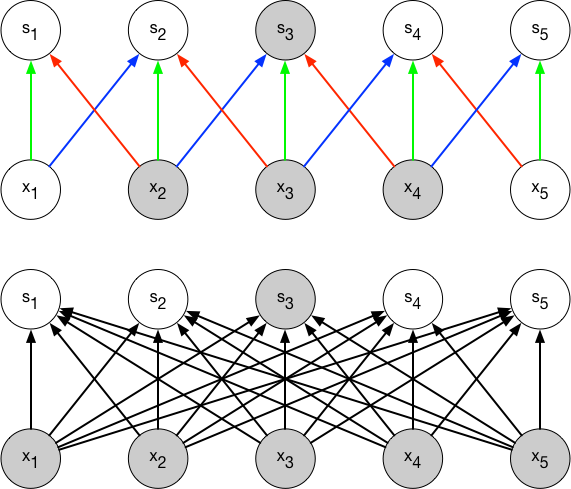
\includegraphics[width=0.6\textwidth]{assets/conv_1d.png}
	\caption{(\textit{Oben})1D Convolution mit \textit{kernel} der Grösse 3. $s_3$ wird durch 3 inputs beeinflusst.
		     (\textit{Unten}) \textit{Dense Network}. $s_3$ wird durch alle inputs beeinflusst.\parencite{goodfellow}}
	\label{img:conv}
\end{figure}

Ein weiterer Vorteil von \textit{Convolutional Neural Networks} ist, dass sie eine räumliche Hyrarchie von Mustern erlernen können. Wenn die Eingabe das Bild einer Katze ist, wird zum Beispiel die erste Schicht unterschiedliche Kanten erkennen, die zweite Schicht dann einzelne Merkmale (z.b Augen), und so weiter.

Damit das gilt, muss aber der analysierte Bereich eines Knotens, von Schicht zu Schicht grösser werden. Deshalb wird meisten nach jedem \textit{Convolution Layer} ein \textit{Pooling Layer} gesetzt. Das \textit{Pooling Layer} fasst mehrere Datenpunkte zusammen um dem nächsten Netzwerk eine grösseren Analysebereich zu verschaffen. Ein oft verwendetes Pooling-Verfahren ist \textit{Max-Pooling}: Angrenzende Knoten werden zusammengefasst durch ihr Maximum. \index{Max-Pooling}
\begin{figure}[hbt]
	\centering
		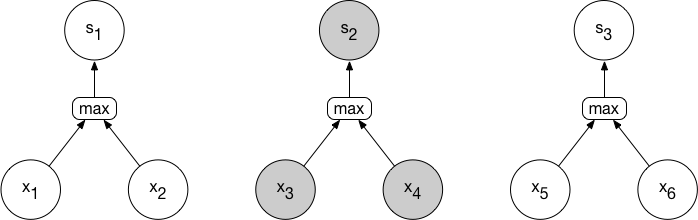
\includegraphics[width=0.75\textwidth]{assets/pooling_1d.png}
	\caption{1D Max-Pooling layer: z.B $s_2$ ist $\max (x3, x4)$}
	\label{img:pool}
\end{figure}


\subsection{Recurrent Neural Networks}
Eine gemeinsame Eigenschaft von allen \textit{Dense Neural Networks} und CNN's ist, dass sie keinen Speicher haben. Bei jedem Vorwärtspass berechnet das Netzwerk alles von neuem, ohne Erinnerungen an vorherige Durchlaufe. Dieses Verhalten ist das absolute Gegenteil vom menschlichem Denkprozess. Wenn wir einen Satz lesen, durchgehen wir ihn Wort nach Wort und merken uns den vorherigen Kontext.

\textit{Recurrent Neural Networks} (RNN) bilden diesen Prozess vereinfacht nach. Sie besitzen eine interne wiederkehrende Schleife die dem Netzwerk Informationen aus dem vorherigen Durchlauf bereitstellt (Siehe Abbildung \ref{img:rnn_loop}). Die RNN Zelle berechnet dann die nächste Ausgabe, sowohl aus der neuen Eingabe, wie auch mit den Erinnerungen der letzten Ausgabe. \parencite{chollet}\\
\begin{figure}[hbt]
	\centering
		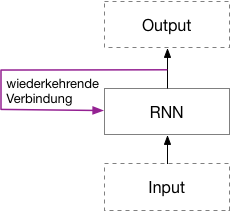
\includegraphics[width=0.35\textwidth]{assets/rnn_loop.png}
	\caption{RNN mit Schlaufe}
	\label{img:rnn_loop}
\end{figure}

Der Vorgang lässt sich grafisch über die Zeit aufgerollt darstellen (Abbildung \ref{img:rnn_unrolled}). In dieser Darstellung fällt auf, dass das Netzwerk theoretisch für jeden Schritt eine Ausgabe besitzt. Die zwischenliegenden Ausgaben sind vor allem wichtig, wenn man eine weitere Schicht an das Netzwerk anhängen will. In der Regel behält man meist nur die letzte Ausgabe, da diese indirekt Informationen über alle anderen beinhaltet.\\
\begin{figure}[hbt]
	\centering
		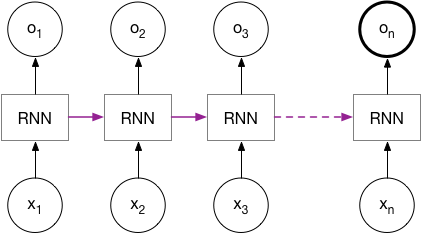
\includegraphics[width=0.67\textwidth]{assets/rnn_unrolled.png}
	\caption{RNN aufgerollt über die Zeit}
	\label{img:rnn_unrolled}
\end{figure}

Das ganze Prinzip ergibt jedoch nur Sinn, wenn frühere Eingaben tatsächlich einen Einfluss auf spätere Ausgaben haben. Eine praktische Anwendung ist das Verarbeiten von zeitlichen Sequenzen, wie Wetterdaten und Sprache. Die einzelnen Lernbeispiele werden  zeitlich zerteilt und stückweise dem Netzwerk gefüttert.
Eine fortgeschrittene Implementation von RNN Zellen ist unter anderem die \textit{Gated recurrent unit} (GRU)\parencite{gru}. Durch das Einführen von unterschiedlichen wiederkehrenden Verbindungen wird verhindert, dass ältere Signale langsam verschwinden, bzw. vergessen werden \parencite{chollet}.